% Created 2026-11-19 Thu 15:02
% Intended LaTeX compiler: pdflatex
\documentclass[10pt,presentation]{beamer}
\usepackage[utf8]{inputenc}
\usepackage[T1]{fontenc}
\usepackage{graphicx}
\usepackage{longtable}
\usepackage{wrapfig}
\usepackage{rotating}
\usepackage[normalem]{ulem}
\usepackage{amsmath}
\usepackage{amssymb}
\usepackage{capt-of}
\usepackage{hyperref}
\usetheme{metropolis}
\usecolortheme{default}
\author{Charlie Zhang}
\date{\today}
\title{Hot Reload for Kotlin/Wasm}
\subtitle{(Fast) Live image development}
\addtobeamertemplate{title page}{}{\vskip-14pt}
\usepackage{tikz}\usetikzlibrary{arrows.meta,positioning}
\usepackage{alltt}
\usepackage{listings}
\lstdefinelanguage{kotlin}{morekeywords={fun,val,var,if,else,for,while,return,when,class,object,interface,companion,override,open,is,in,Int,Long,Short,Byte,Char,Boolean,Unit,Float,Double,String},sensitive=true,morecomment=[l]{//},morecomment=[s]{/*}{*/},morestring=[b]"}
\lstset{basicstyle=\ttfamily\small,keywordstyle=\bfseries,commentstyle=\itshape\color{black!55},showstringspaces=false}
\hypersetup{
 pdfauthor={Charlie Zhang},
 pdftitle={Hot Reload for Kotlin/Wasm},
 pdfkeywords={},
 pdfsubject={},
 pdfcreator={Emacs 30.2 (Org mode 9.7.11)}, 
 pdflang={English}}
\begin{document}

\maketitle
\begin{frame}{Outline}
\tableofcontents
\end{frame}

\section*{Background}
\label{sec:org9668bbf}
\begin{frame}[label={sec:orga539dc6},fragile]{What is hot reload?}
 \begin{itemize}
\item Edit code \(\Rightarrow\) immediate reload feedback without restarting the
application
\begin{itemize}
\item Most importantly, the state survives
\item e.g. scroll position, navigation stack, half-filled form.
\end{itemize}
\item In the context of a typical Kotlin/Compose workflow, saving a \texttt{.kt}
file under hot-reload will instantly update your webapp with those
changes without throwing away the state.
\item This kind of on-the-fly code redefinition in the running image also
underpins classical REPLs a la Lisp, Smalltalk.
\end{itemize}
\end{frame}
\begin{frame}[label={sec:org9efc8f9}]{What's out there?}
\begin{center}
\footnotesize\setlength{\tabcolsep}{3pt}
\begin{tabular}{lll}
System & Mechanism & Allowed changes\\
\hline
JVM HotSwap & bytecode replacement & method bodies only\\
JVM agents / DCEVM & class redefinition (Live Edit) & bodies + limited shape\\
Vite / React Fast Refresh & module swap + runtime hooks & per-component rules\\
Flutter hot reload & tree rebuilt over state & most state\\
Lisp / Smalltalk images & late binding for everything & everything\\
\end{tabular}
\end{center}

\begin{itemize}
\item The motivating case for us: \alert{Compose}. UI iteration is dominated by
the edit \(\to\) save \(\to\) compile \(\to\) reload \(\to\) display loop; JetBrains
ships Compose Live Edit on the JVM because having this feedback loop
short makes development productive and \alert{fun}.
\begin{itemize}
\item Waiting for the compiler and reconstructing state breaks flow state.
\item \(\Rightarrow\) The demand is real.
\end{itemize}
\end{itemize}
\end{frame}
\begin{frame}[label={sec:org40a0f8f}]{Requirements}
\begin{enumerate}
\item \alert{Edit-to-screen under a second} from real file saves
\item \alert{State survival}: data/objects persist even when the
behavior/classes they belong to change. No application restarts.
\item \alert{Graceful error handling}: a rejected change due to e.g. compiler
errors or traps shows an error overlay while the app keeps running
the old code
\item Works with the user's existing dev environment.
\begin{itemize}
\item Most simple generic form is reload on editor save.
\end{itemize}
\end{enumerate}
\end{frame}
\section*{Previous and preliminary work}
\label{sec:org14f79e2}

\begin{frame}[label={sec:org8b951f4}]{Recently developed prerequisites}
\begin{itemize}
\item Igor prototyped a version of hot-reload for Wasm \textasciitilde{}2 years ago
\begin{itemize}
\item Could do things like method redefinitions, but hacked together
\end{itemize}
\item Since then, 3 important features independent of hot-reload mainlined
for Wasm that are a requirement for \alert{short dev loops} (issue 1).
\begin{enumerate}
\item \alert{Multi-module compilation}
\item \alert{Stable signatures}
\item \alert{Wasm incremental compilation}
\end{enumerate}
\item Together, these allow us to speed up the dev loop by allowing us to
create small modules containing only code that is added or changed,
while importing dependencies from existing modules.
\item Independent of state survival: you can imagine a hot reload where
the whole application is recompiled into a single module as long as
loading preserves state, but this can take a long time.
\end{itemize}
\end{frame}
\begin{frame}[label={sec:org2ce6482}]{Multi-module compilation}
\begin{itemize}
\item Allows one compilation to emit several wasm modules, with
declarations imported across module boundaries.
\item Without this, we'd only be able to hot-reload one large monolith
containing the entire program, including the stdlib and all other
libraries, every time.
\end{itemize}
\end{frame}
\begin{frame}[label={sec:org08edd6b}]{Stable signatures}
\begin{itemize}
\item Makes every declaration carry a cross-compilation identity that
survives klib serialization and orders type emission
\item For Wasm, it means type rec groups are emitted deterministically and
ordered by stable signature, so two independently compiled modules
declaring the same class emit \alert{byte-identical} type sections.
\item V8 canonicalizes identical rec groups into one runtime type:
\alert{type identity across separately compiled modules}.
\item Without this, it would be difficult for the engine to know that
objects across different modules are the same and it would be
difficult to type-check values crossing module boundaries.
\end{itemize}
\end{frame}
\begin{frame}[label={sec:org75228f6}]{Incremental compilation (Wasm IC)}
\begin{itemize}
\item Allows only compiling parts of the program that have changed since
the last compilation via use of per-file lowered fragments, cached,
with precise dirty set.
\item Whereas multi-module compilation allows loading individual modules
of Wasm code, IC allows detecting differences in source and only
compiling sources that have changed.
\item Inline functions are content-hashed — a changed inline dirties all
its \alert{callers' files} too (exactly the propagation semantics hot
reload needs).
\item Without this, we would not know which files need to be recompiled
when the sources change and how to handle inlining correctly either.
\begin{itemize}
\item Avoids re-lowering non-dirty files, even if their IRs are needed
for linkage/other resolution purposes (think types etc).
\end{itemize}
\end{itemize}
\end{frame}
\section*{Coordinating the compiler server}
\label{sec:orgcfe4cb0}

\begin{frame}[label={sec:org54bc011}]{In-image compilation or compiler server?}
\begin{itemize}
\item We don't have in-image K2wasm compiler in the browser.
\begin{itemize}
\item Possible in theory; we haven't tried it.
\end{itemize}
\item No in-image loader: V8 exposes nothing that links or patches modules
from inside a module: New Wasm code must be loaded from the
environment host (JS for wasm/js).
\item Current solution: send Kotlin code to a JVM Kotlin compile server,
ship the resulting wasm module to the host to get loaded in the
running image.
\end{itemize}
\end{frame}
\begin{frame}[label={sec:orge876240}]{Pros and cons}
\alert{Pros}

\begin{itemize}
\item No compiler in the browser needed
\begin{itemize}
\item Saves on download, compiler bootstrap; the image self-hosts
\alert{runtime} machinery only
\end{itemize}
\item Reuses existing daemon + IC stuff
\item The compiler can keep heavyweight state (analysis, PSI, caches) that
would never fit the page
\end{itemize}

\alert{Cons}

\begin{itemize}
\item An extra trip on every edit: the delta bytes must cross the wire
\item The compiler is not itself hot-reloadable
\begin{itemize}
\item Misses out on Lisp-style hack on the compiler while using the
compiler.
\end{itemize}
\item The compiler doesn't know about the state of the live image
\begin{itemize}
\item Compatibility issues are discovered at load time/run time, not
diagnosed at compile time.
\end{itemize}
\end{itemize}
\end{frame}
\section*{Compiler work: Making the runtime and codegen redefinition amenable for state survival}
\label{sec:org647bbfc}

\begin{frame}[label={sec:orgbf0cb6b}]{Wasm-specific challenges for state survival}
\begin{itemize}
\item A wasm module is immutable once validated; an instance is frozen
w.r.t its imports + globals + code addresses.
\item No JVM-style class redefinition exists in Wasm: there is no engine
API that replaces a function body or a struct type inside a live
instance.
\item The \alert{only} thing an engine lets you do is instantiate \alert{more} modules
and load them into the host runtime (e.g. V8, wasi runtimes, etc)
\item So: we need a lot of code generation support from the compiler
backend to do redefinition.
\begin{itemize}
\item Only thing we can do: compile new code into modules, load it into
the existing process/image via the host, coordinate the
loader/runtime to overwrite existing behavior (somehow)
\end{itemize}
\end{itemize}
\end{frame}
\begin{frame}[label={sec:orgbed6dab},fragile]{Existing codegen}
 \begin{itemize}
\item Normally, the wasm backend emits calls with eager linkage - \texttt{call
  \$f} addresses the function's own module or through its own module's
imports.
\item Modules are sealed: a mutable global, an object, or a slot \emph{cannot
move} between instances.
\item So already loaded functions can never call newly loaded code or be
redefined themselves.
\item Classes pose even more of a problem for redefinition: their types
are translated into wasm structs where everything is strongly typed
and the layout fixed ahead of time.
\begin{itemize}
\item Object getters/setters/type tests fixed against these types in the
bytecode.
\item No JVM-like solution exposed on the engine level for bytecode
replacement.
\end{itemize}
\end{itemize}
\end{frame}
\begin{frame}[label={sec:org4df60ee},fragile]{Make everything indirect}
 \begin{itemize}
\item Solution: We can add a new compilation mode that changes low-level
codegen to make everything redefinable
\begin{itemize}
\item with \texttt{-Xwasm-hot-reload} we can have the dynamic language of our
dreams
\end{itemize}
\item Main affected pieces:
\begin{itemize}
\item Function/method redefinition (indirect linkage with lazy
resolution)
\item Class redefinition (indirect layouts with lazy obsolete instance
migration)
\end{itemize}
\item Borrow implementation ideas heavily from Lisp/Smalltalk codegen and
runtime support where they do precisely this: everything is
redefinable inside a running image.
\begin{itemize}
\item Additionally, figure out how to map those ideas to a
strongly-statically-typed bytecode world.
\end{itemize}
\end{itemize}
\end{frame}
\begin{frame}[label={sec:orgd55c739}]{High level overview of new machinery}
\begin{itemize}
\item Wrap all function calls through an indirect function \alert{cell}.
\begin{itemize}
\item At module-load time, the module initializer looks up the function
cell by name and writes the new funcref into the cell.
\end{itemize}
\item Similarly, separate structs representing classes into layout
metadata and field payload data.
\begin{itemize}
\item Objects are then wrapped with indirections to runtime descriptions
of the classes they belong to and field payload data.
\item Layouts are `metaclass` Wasm structs describing object layouts and
keyed by name in the image
\item At module-load time, the module initializer handles class
redefinitions by invalidating old layouts which causes existing
objects to migrate to their new layouts lazily
\end{itemize}
\item Notably, these indirection cells/layouts are first-class GC objects,
so they can cross module instance boundaries and be shared
\end{itemize}
\end{frame}
\begin{frame}[label={sec:orgd96c8e4},fragile]{A running example: fun double}
 \begin{verbatim}
fun double(n: Int): Int = n * 2  // module A: the callee

fun render(): String =           // module B: a caller
    "count: ${double(21)}"

val held: (Int) -> Int = ::double  // funcref in a val
\end{verbatim}

\begin{itemize}
\item \texttt{render}'s call and \texttt{held}'s funcref are callers of \texttt{double}
\item The next slides show what \texttt{double} compiles to and what happens when
a new module redefines it live.
\item Methods work in the same way as top-level functions.
\end{itemize}
\end{frame}
\begin{frame}[label={sec:orga7568a5},fragile]{Indirect linkage: function cells}
 \begin{verbatim}
;; the function cell type: called fdefn:
(type $fdefn (sub (struct (field $fn (mut funcref)))))
;; double's signature type (real output: anonymous):
(type $sig_double (func (param i32) (result i32)))
\end{verbatim}
\begin{itemize}
\item The stdlib keeps a \texttt{HashMap<String, fdefn>} table in the running
image
\begin{itemize}
\item Exposes some functions to register and lookup \texttt{fdefn} s.
\end{itemize}
\item Every call of \texttt{double} in a module goes through a module-global
holding the callee's cell.
\item The module initializer resolves the cell at load and creates it on
first definition.
\end{itemize}
\end{frame}
\begin{frame}[label={sec:org5d75e77},fragile]{Indirect linkage: function cells (cont.)}
 \begin{verbatim}
;; the cell global (will be overwritten at load time)
(global $__hot_cell$double#4f2a (mut (ref null $fdefn))
  ref.func $double struct.new $fdefn)

;; an entry stub is registered under double's real key:
(func $__hot_entry$double#4f2a (param i32) (result i32)
  local.get 0
  global.get $__hot_cell$double#4f2a
  struct.get $fdefn $fn
  ref.cast (ref $sig_double)  ;; per-call type check
  call_ref $sig_double)

;; render's call site is just an ordinary call:
...
  call $__hot_entry$double#4f2a
\end{verbatim}

\begin{itemize}
\item Vtable slots and funcrefs are just \texttt{ref.func} of the entry stub.
\end{itemize}
\end{frame}
\begin{frame}[label={sec:org04ff952},fragile]{The redefinition, step by step}
 \begin{itemize}
\item \alert{At save}: \texttt{fun double(n: Int) = n * 4} compiled to new module C
\item \alert{At load}: C's init resolves \texttt{"double\#4f2a"} against the image: it
finds A's SHARED cell and installs C's impl via one \texttt{struct.set}.
The new body is live once loading finishes
\item \alert{Unchanged and unaware}: every caller (e.g. \texttt{render}'s call site,
the funcref \texttt{held}, any vtable slots) resolves to the entry, which
reads the cell per call. No need to patch anything.
\item \alert{A different signature?} Creates a new overload with its own name
and cell; old callers untouched. (Like in Julia).
\end{itemize}
\end{frame}
\begin{frame}[label={sec:orgccc879c}]{Making classes runtime redefinable}
\begin{itemize}
\item With wasm, objects of a struct type are frozen to a given layout;
wasm GC subtyping can only \alert{extend} field lists, and types are
canonicalized by content.
\item What we want: old instances keep working, new code sees new fields,
and identity survives.
\item The naive solution of redeclaring with extra fields breaks type
identity across modules; old objects are stuck with the old
(obselete) type.
\item The rest of this section follows one example class through the hot
reload machinery that solves these issues.
\end{itemize}
\end{frame}
\begin{frame}[label={sec:orgccf1a3d},fragile]{An example: class Model}
 \begin{verbatim}
class Model(val label: String, val count: Int) {
    var hits = 0
    fun bump() { hits++ }
}
\end{verbatim}

\begin{itemize}
\item Imagine adding a new field \texttt{val name: String}
\begin{itemize}
\item Existing instances \alert{must} keep their state and identity.
\end{itemize}
\item The compiler will have to create a new module with a new class
definition that can be reloaded and effect old \texttt{Model} objects.
\end{itemize}
\end{frame}
\begin{frame}[label={sec:orgde831bf},fragile]{Runtime layouts}
 \begin{itemize}
\item We add a runtime descriptor called a layout that describes a class
\begin{itemize}
\item It itself is an ordinary stdlib Kotlin class containing:
\begin{itemize}
\item the class's current vtable + itable
\item an \texttt{allocate} closure responsible for creating a payload
structure with the shape of the layout described by this
descriptor. Only the defining module can build the layout
because type signatures can't be created at runtime, so the
closure is built in the same module.
\item a vector of slot (field) descriptions of \texttt{HotSlot\{nameTag,
      typeTag, reader, writer\}}
\item Tags are the slot's name hash + type tag
\end{itemize}
\end{itemize}
\item For \texttt{Model}, the slot vector is \texttt{label}, \texttt{count}, \texttt{hits}
\begin{itemize}
\item This runtime information is what lets existing objects migrate
lazily to new class definitions.
\end{itemize}
\item Terminology note: The word field is a bit overloaded in this case
because they also describe Wasm type fields
\begin{itemize}
\item I use slot to mean a Kotlin field.
\end{itemize}
\end{itemize}
\end{frame}
\begin{frame}[label={sec:org47af6a8},fragile]{The structs (1/2): cell and payload}
 \small
\begin{verbatim}
// the CELL — every object's stable shape
struct Model {
  VTable  vtable;     // root-typed, mutable
  ITable  itable;
  Rtti    rtti;
  Payload payload;    // root-typed, mutable
}

// the PAYLOAD — Model's fields, swappable in place
struct Model$payload {
  int       _hashCode;
  HotLayout *$layout;   // stamped at birth
  String    label;
  int       count;
  int       hits;
}
\end{verbatim}
\normalsize
\end{frame}
\begin{frame}[label={sec:orgc9d580d},fragile]{The structs (2/2): layout and slot}
\small
\begin{alltt}
// the LAYOUT — the runtime class descriptor
struct HotLayout \{
  VTable  vtable;     // the CURRENT dispatch half
  ITable  itable;
  Rtti    rtti;       // interface gains stay hot
  funcref allocate(); // allocares a payload of this shape
  HotSlot slots[];    // one per field
\}

// the SLOT descriptor:
struct HotSlot \{
  long    nameTag;    // the slot's name hash
  long    typeTag;    // its type's class identity
  funcref reader;     // (anyref) \ensuremath{\to} anyref
  funcref writer;
\}
\end{alltt}
\normalsize
\end{frame}
\begin{frame}[label={sec:org55ff7d0},fragile]{Class representation in Wasm}
 \begin{verbatim}
(type $Any$payload  ;; the ROOT payload
  (sub (struct (field $_hashCode (mut i32))
       (field $$layout (ref null $HotLayout)))))
(type $Model (sub $AnyCell
  (struct ...vtable/itable/rtti...
    (field (mut (ref null $Any$payload))))))
\end{verbatim}
\begin{itemize}
\item All types like \texttt{\$Model} are subtypes of the \alert{cell} containing
\texttt{\{vtable, itable, rtti, payload\}}
\begin{itemize}
\item Invariant under redefinition.
\end{itemize}
\item The payload field is mutable, typed at the \alert{root} payload type
holding a pointer to a layout
\begin{itemize}
\item The layout is hence reachable from \alert{any} object, without knowing
what type to cast to.
\end{itemize}
\item Reading a field then means casting to a specific payload type and
calling \texttt{struct.get}.
\begin{itemize}
\item See Step 3 for the emitted form.
\end{itemize}
\end{itemize}
\end{frame}
\begin{frame}[label={sec:org27f9a17},fragile]{Class tutorial: the map}
 With this encoding in place, the following six steps will demonstrate
what happens to the class (running example: \texttt{Model}):

\begin{enumerate}
\item \alert{compile \& load}: creates the cell + payload + per-slot closures
for the module; loading registers the layout in the image's layout
table
\item \alert{allocate}: stamp \texttt{\$layout} into the fresh payload
\item \alert{access}: \texttt{ref.test} fast path; a miss does a dynamic lookup
\item \alert{redefine \& migrate}: the next load replaces the layout;
updateInstance on the first stale access (step 6)
\item \alert{old code}: reads by name through the image
\item \alert{dispatch}: if obsolete vtable / itable / RTTI, then
migrate. retry.
\end{enumerate}

You can see that migration is lazy (on-first access).

Upshot: \alert{old instances keep working, new code sees new fields,
identity survives.}
\end{frame}
\begin{frame}[label={sec:orgd6f4ae4},fragile]{Step 1 — compile \& load}
 \begin{verbatim}
;; per class, at load (the module's init):
layout = image.hotLayoutsRegister(classId,
    vtable, itable, rtti, allocate)
image.hotLayoutsAddSlot(classId,   ;; per field:
    nameTag, typeTag, reader, writer)
layoutGlobal$Model = layout  ;; module-local
\end{verbatim}
\begin{itemize}
\item The cell type, payload struct (keyed by class), and per-slot
closures with erased signatures (reader, writer, allocator) compiled
into the module
\begin{itemize}
\item The concrete casts live \alert{inside} each closure like with fdefn entries.
\end{itemize}
\item Load time registers these in the image by setting the current layout
in a map from classId \(\to\) current layout.
\begin{itemize}
\item Similar to the fdefinition map.
\end{itemize}
\item Putting RTTI's in the layout allows us to dynamically add interface
supertypes as well.
\end{itemize}
\end{frame}
\begin{frame}[label={sec:orgcdf3ce5},fragile]{Step 2 — allocation stamps the layout}
 \begin{alltt}
;; allocation: struct.new $payload, then
$layout \ensuremath{\leftarrow} layoutGlobal$Model   ;; one instruction
;; \ensuremath{\to} every instance names its own payload shape
\end{alltt}

\begin{itemize}
\item Every allocation stamps the payload's \texttt{\$layout} from the module's
layout global. Since the field is \alert{root}-typed, any code reaches the
layout with one \texttt{struct.get} without a cast needed first.
\item A module that only instantiates a class defined elsewhere (like from
the stdlib) need no layout global for it, load-time just asks the
image for the class's current layout.
\item For bootstrap, the classes defining this machinery (layout is a
Kotlin class for example) get null layouts (redefining the layout
class themselves would cause a vicious meta-circle).
\begin{itemize}
\item Irrelevant for application developer.
\end{itemize}
\end{itemize}
\end{frame}
\begin{frame}[label={sec:orga5db04b},fragile]{Steo 3 - fast field access, with fallback}
\begin{alltt}
local.get $cell
struct.get $Any 3            ;; payload, root-typed
ref.test (ref $payload$Model)
if  ;; fast path: payload is the current layout's payload
  ref.cast; struct.get       ;; inline access
else ;; slow: dynamic lookup
  $cell, nameTag, typeTag \ensuremath{\to} slotValue
end
\end{alltt}

\begin{itemize}
\item For simple field addition redefinitions, the fast path is also
reached, since we use subtyping in that case.
\item The slow path triggers migration (the payload gets swapped out), so
future accesses will be fast.
\end{itemize}
\end{frame}
\begin{frame}[label={sec:orge29f01f},fragile]{Step 4 — redefinition \& migration}
\begin{alltt}
updateInstance(cell, classId, to):
  from = payload.$layout        ;; EQ identity
  if from !== to:               ;; shapes differ
    fresh = to.allocate()  ;; news the new shape
    copy _hashCode + same-named,
      same-TAGGED slots: reader \ensuremath{\to} writer
    cell.payload = fresh        ;; swap IN PLACE
\end{alltt}

\begin{itemize}
\item Migration entered through slow path access.
\begin{itemize}
\item Code to do so is just normal stdlib kotlin.
\end{itemize}
\item Accessor funcrefs come from the defining module since that's where
the static types are.
\item A retyped slot is \alert{not} copied, since a copy would trap the writer's
cast mid-migration; it just takes its type default, everything else
migrates cleanly
\begin{itemize}
\item Could also make the field do its initializer (not done yet)
\end{itemize}
\item \alert{One shot, in place}: the cell is never reallocated, so identity
never changes.
\end{itemize}
\end{frame}
\begin{frame}[label={sec:org54a60b1},fragile]{Redefinition, diagrammed (add \texttt{val name: String})}
 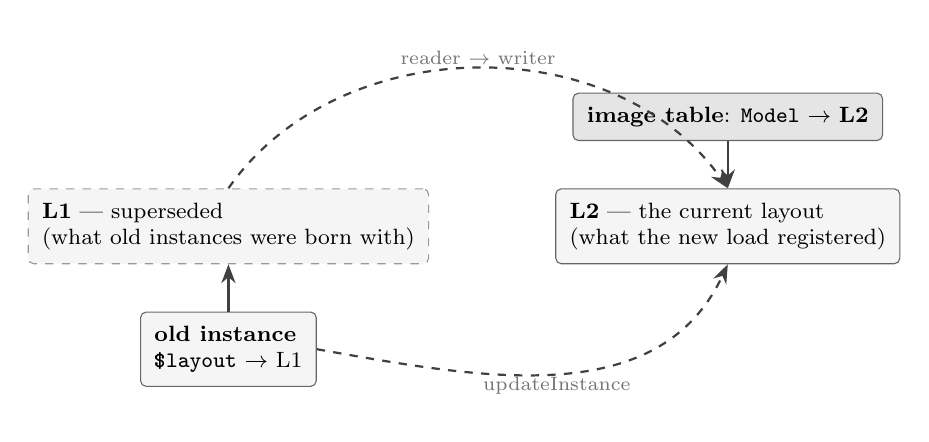
\begin{tikzpicture}[
  font=\footnotesize,
  box/.style={draw=black!60, rounded corners=2pt, inner sep=5pt, align=left, fill=black!4},
  arr/.style={-{Stealth[length=2.4mm]}, black!75, thick},
  lbl/.style={font=\scriptsize, text=black!55, align=center, inner sep=1pt},
]
\node[box, fill=black!10] (table)
  {\textbf{image table}: \texttt{Model} $\to$ \textbf{L2}};
\node[box, below=6mm of table] (l2)
  {\textbf{L2} — the current layout\\ (what the new load registered)};
\node[box, left=16mm of l2, draw=black!40, dashed] (l1)
  {\textbf{L1} — superseded\\ (what old instances were born with)};
\node[box, below=6mm of l1] (old)
  {\textbf{old instance}\\ \texttt{\$layout} $\to$ L1};
\draw[arr] (table) -- (l2);
\draw[arr] (old) -- (l1);
\draw[arr, dashed] (l1.north) to[out=55,in=125]
  node[above, lbl] {reader $\to$ writer} (l2.north);
\draw[arr, dashed] (old.east) to[out=-10,in=-115]
  node[below, lbl] {updateInstance} (l2.south);
\end{tikzpicture}

\begin{itemize}
\item Old instances keep L1 until first stale access; new allocations
stamp L2.
\item \texttt{L2 = L1} plus the \texttt{name} slot: the copy runs reader \(\to\) writer
per shared slot (here: added \texttt{name} with a type-default \texttt{""})
\begin{itemize}
\item Since the slot lists are computed at \alert{runtime}, the compiler
doesn't need to know about how things used to be just to emit the
right static types to bytecode for migration.
\end{itemize}
\end{itemize}
\end{frame}
\begin{frame}[label={sec:org6fec78e},fragile]{Step 5 — old code reads by name}
 \begin{itemize}
\item A dynamic call to \texttt{hotLayoutsSlotValue(cell, nameTag, typeTag)}
derives the \alert{concrete} class from the instance's RTTI klassId and
migrates if it is stale.
\begin{itemize}
\item Reads the slot and returns the value by looking up the associated
reader closure through the current layout through the current
layout and calling it.
\end{itemize}
\item The lookup is done by tags: \texttt{nameTag} is the slot's name hash;
\texttt{typeTag} is its type's class identity plus a nullability bit
\begin{itemize}
\item tag-equal means cast-compatible by construction.
\end{itemize}
\item A deleted or retyped slot \alert{throws a catchable exception} ("unbound
slot")
\begin{itemize}
\item The field is gone, not shadowed.
\end{itemize}
\item Function-typed slots
\begin{itemize}
\item A funcref is not an anyref (wasm's func and
\end{itemize}
any hierarchies are disjoint)
\begin{itemize}
\item We can just box the value to make the machinery Wasm type-check
without duplicating the code.
\item Migration then copies the box like with any other slot.
\end{itemize}
\end{itemize}
\end{frame}
\begin{frame}[label={sec:orgdfd6fc3},fragile]{Step 6 — dispatch: migrate, then retry}
 \begin{verbatim}
;; virtual call, emitted:
vtable = cell.vtable
ref.test $vtable_expected
if (pass) cast + call slot
else hotVtableUpdate(cell) ;; then RETRY
\end{verbatim}

\begin{itemize}
\item Migration code reads the RTTI klassId \(\to\) current layout \(\to\)
install(vtable, itable, RTTI)
\begin{itemize}
\item the new grown vtable is a \alert{subtype of the old one}, so the
retry's cast still passes
\item a method added later can still dispatch on old objects defined
before the method existed.
\end{itemize}
\item Interface supertype additions work as well: interfaces erase from
every signature; the RTTI \texttt{id} list and \texttt{itable} slots are just
runtime data.
\begin{itemize}
\item the itable lookup renders null on a stale RTTI, the migrator
installs the \alert{current} RTTI + itable, and the instance answers \texttt{is
    I} and dispatches after one migration.
\end{itemize}
\end{itemize}
\end{frame}
\begin{frame}[label={sec:org6c52856},fragile]{Worked example summary}
 \begin{itemize}
\item \alert{v1}: \texttt{class Model(val label: String, val count: Int)} with a
million live instances.
\item \alert{At save}: Add \texttt{val name: String}
\begin{itemize}
\item A new payload shape is compiled and registered at load:
\texttt{image[Model] = current}
\item Nothing migrates yet.
\end{itemize}
\item \alert{First new-code access}: \texttt{updateInstance} runs when \texttt{ref.test}
misses
\begin{itemize}
\item \texttt{label}, \texttt{count} copied, \texttt{name} defaulted; the payload swapped
\alert{in place}
\item identity kept.
\end{itemize}
\item \alert{Old code}: reads \texttt{label}, count by \texttt{name} through the layout (slow path)
\end{itemize}
\end{frame}
\begin{frame}[label={sec:org993b4b7}]{What each edit does — compatible changes}
\begin{center}
\scriptsize
\begin{tabular}{p{0.16\textwidth} p{0.34\textwidth} p{0.36\textwidth}}
edit & mechanism & old instances\\
\hline
body-only & loader just installs new bodies into the shared cells & run new bodies via vtables\\
add fields & allocagte new payload; the module registers the new layout & migrate lazily on first access (update-instance); identity + values kept\\
add open method & vtable grows (behind the mutable root-typed field) & new method callable on old instances; overrides still win\\
interface default body & the itable installs with the vtable (same migration) & swaps hot on live instances\\
\end{tabular}
\end{center}
\end{frame}
\begin{frame}[label={sec:orgf90fb65}]{What each edit does — incompatible changes}
\begin{center}
\scriptsize
\begin{tabular}{p{0.22\textwidth} p{0.32\textwidth} p{0.32\textwidth}}
edit & mechanism & outcome\\
\hline
delete field / change its type & new payload is a \alert{sibling} (wasm subtyping never shrinks) & migration copies same-named same-typed slots (a retyped slot takes a default); old code touching the changed slot \alert{throws a catchable exception} in the image\\
gain a class supertype, flip finality & the cell chain is part of every signature mentioning the class — the engine rejects the patch's instantiation & old code keeps running; stranded bindings reported\\
\end{tabular}
\end{center}
\end{frame}
\section*{Edge cases}
\label{sec:orgda5e1e5}

\begin{frame}[label={sec:org74ea8ca},fragile]{Top-level properties}
 \begin{itemize}
\item What to do with \texttt{val x = object \{ ... \}}?
\item Compose developers probably just expect the object to gain new
fields/methods or delete old things
\begin{itemize}
\item Not that the object gets created anew because the top-level
property is redefined.
\end{itemize}
\item This is acheived by just migrating fields over with the same
mechanism as before so singletons keep state.
\begin{itemize}
\item Just need the compiler to special case this top-level property on
object shape.
\end{itemize}
\end{itemize}
\end{frame}
\section*{How I developed this}
\label{sec:org66786d6}
\begin{frame}[label={sec:org0a993c6}]{Demo}
\begin{itemize}
\item Everything discussed in these slides is implemented.
\item Demo video in \#kotlin-wasm-internal
\end{itemize}
\end{frame}
\begin{frame}[label={sec:orgbdeeb64}]{GLM is pretty good}
\begin{itemize}
\item It couldn't come up with any of the codegen ideas discussed here
(luckily Lisp exists)
\item But very useful for creating JS scaffolding, compiler changes,
debugging, dealing with gradle for compiler builds.
\begin{itemize}
\item It understands how IC works!
\end{itemize}
\end{itemize}
\end{frame}
\section*{Appendix}
\label{sec:org8ec908e}

\begin{frame}[label={sec:org3b19655},fragile]{The CLOS correspondence (for the Lisp-literate)}
 \begin{center}
\scriptsize
\begin{tabular}{p{0.42\textwidth} p{0.48\textwidth}}
here & Common Lisp (SBCL/AMOP)\\
\hline
cell: shape never changes, identity kept & wrapper split: stable instance, swapped layout\\
the payload: swappable slot vector, \texttt{\$layout} stamped at birth & PCL's instance body: wrapper pointer + slot vector\\
the LAYOUT: vtable, itable, slot descriptors, accessor closures — registered in the image & SBCL's wrapper with the indirection removed: identity and layout fused in one object\\
no shape naming: payload keyed by class; identical shapes unify by content & a redefinition is an event, not content; healing is just a full copy\\
update-instance: allocate, copy same-tagged slots, swap in place — one shot & \texttt{update-instance-for-redefined-class} — lazy, never eager\\
slot-value by name; deleted slot throws catchable & obsolete code touching a discarded slot errors; no shadow reads\\
\end{tabular}
\end{center}

\begin{itemize}
\item The one divergence: CL layouts add \alert{and drop} slots freely; wasm GC
subtyping can only extend — deletions mint \alert{sibling} payloads; the
catchable unbound-slot is the old-code story.
\end{itemize}
\end{frame}
\end{document}
